\documentclass{article}

% Language setting
% Replace `english' with e.g. `spanish' to change the document language
\usepackage[russian]{babel}
\usepackage{tcolorbox}
\usepackage{caption}
\usepackage{subcaption}
% Set page size and margins
% Replace `letterpaper' with `a4paper' for UK/EU standard size
\usepackage[letterpaper,top=2cm,bottom=2cm,left=3cm,right=3cm,marginparwidth=1.75cm]{geometry}

% Useful packages
\usepackage{amsmath}
\usepackage{amssymb}
\usepackage{graphicx}
\usepackage{fixltx2e}
\usepackage[colorlinks=true, allcolors=blue]{hyperref}

\title{Quantitative Analytics.\\
Lectures. Week 1. \\
The Black-Scholes-Merton model}
\author{Vorontsov Daniil}
\date{\today}
\begin{document}
\maketitle
\setcounter{tocdepth}{1} % {2} - в оглавлении участвуют chapter, section и subsection. {1} - только chapter и section
\renewcommand\contentsname{Contents}
\tableofcontents
\newpage\textbf{Модель Блэка-Шоулза-Мёртона (БШМ)} (англ. \textit{Black–Scholes-Merton}) используется для оценки цены на классический (ванильный) европейский опцион.

\section{Логнормальное распределение}
Одно из предположений модели Блэка-Шоуза-Мёртона состоит в том, что стоимость базового актива (БА) подчинена \textbf{логнормальному} распределению. Что это значит?\\

Предположим, что возвратная инвестиция в какую-то акцию подчинена \textbf{нормальному} распределению:\\
\begin{equation}
    \frac{\Delta S}{S}\sim\varphi(\mu\Delta t, \sigma^{2}\Delta t)
\end{equation}
Здесь $\mu -$ матожидание доходности, $\sigma - $волатильность цены акции.\\
В предположении независимости приращений из уравнения (1) можно математически вывести:
\begin{equation}
    lnS_t\sim N(lnS_0+(\mu - \frac{\sigma^2}{2})T, \sigma^2T)
\end{equation}
То есть логарифм $S_t$ распределён нормально, или же сама величина распределена лог-нормально. Здесь обозначения:\\
$S_t -$ цена акции в момент времени $T$\\
$S_0 -$ цена акции в момент времени $t=0$\\
$\mu -$ ожидаемый доход с акции за год\\
$\sigma -$ волатильность акции за год\\
У распределения (2) следует обозначить ряд свойств:
\begin{itemize}
    \item Суммарный(кумулятивный) годовой доход с акции\footnote{Прим. здесь имеется в виду \textit{compound annual return} - общая сумма дохода от инвестиции, когда начисляемый процент используется на увеличение суммы инвестиции, т.н. "сложный процент" (vocable.ru/termin/compound-annual-return.html)} $x$ распределён нормально с параметром матожидания $\mu - \frac{\sigma^2}{2}$ и параметром дисперсии $\frac{\sigma^2}{T}$:\\
    $x\sim\varphi(\mu-\frac{\sigma^2}{2},\frac{\sigma^2}{T})$
    \item $\mathbf{E}[S_t] = S_0 e^{\mu T}$
    \item \mathbf{Var}($S_t$)=$S_0^2e ^{2\mu T}(e^{\sigma^2 T}-1)$
    \item Матожидание доходности на малом промежутке $\Delta t$ : $\mu$, на момент времени $T: \mu-\frac{\sigma^2}{2},\frac{\sigma^2}{T}$
    \item Средняя доходность всегда будет чуть меньше матожидания из-за стохастической компоненты.
\end{itemize}

\section{Расчёт исторической волатильности}
Как рассчитать волатильность БА? По одному из определений, волатильность - стандартное отклонение суммарного годового дохода (из свойств формулы (2): $\frac{\sigma}{\sqrt{T}}$)

В предположении о том, что случайная величина распределена на более длинном периоде аналогично короткому, можно вывести волотильность за нужный период как $\sigma \sqrt{N}$, где $N -$ кол-во периодов.

Процесс расчёта исторической волатильности состоит в сборе данных дневных котировок цен $S_i$, получении серии соответствующих доходов $ln(\frac{S_i}{S_{i+1}})$ и расчёте методами математической статистики стандартного отклонения данного временного ряда. Годовая волатильность получается домножением отклонения на корень из кол-ва дней, в которые велась торговля в этом году.

Пример расчёта:
\begin{enumerate}
\item Конвертация $N+1$ дневных цен в $N$ доходов: $R_i=\frac{S_i-S_{i-1}}{S_{i-1}}$
\item Расчёт суммарного дохода $R_i^c=ln(1+R_i)=ln(\frac{S_i}{S_i-1})$
\item Расчёт дисперсии $\sigma^2=\frac{\sum(R_i^c-\overline{R}_i^c)^2}{N-1}$
\item Получение корня из дисперсии $s=\sqrt{\frac{1}{N-1}\sum(R_i^c-\overline{R}_i^c)^2}$
\item Получение отклонения как $\hat{\sigma}=\frac{s}{\sqrt{\tau}}$, где $\tau$ интервал в годах (для годового отклонения $\tau=\frac{1}{12}$, для недельного $\tau=\frac{1}{52}$)
\end{enumerate}


\section{Предположения модели БШМ}
В основе модели БШМ лежат 8 предположений:
\begin{enumerate}
\item БА подчинён логнормальному распределнию (на коротком промежутке времени)
\item Отсутствие арбитража: если появляется возможность арбитража, моментально элиминируется участниками торгов
\item Волатильность БА постоянна и известна
\item Отсутствуют транзакционные комиссии, налоги. БА бесконечно делимый
\item На БА отсутствуют денежные потоки (не приходят дивиденды)
\item Торговля ведётся непрерывно
\item Безрисковая процентная ставка постоянна
\item Исполнение опциона возможно в определённую контрактом дату. Иными словами, рассматриваются только Европейские опционы
\end{enumerate}\\
При этом некоторые предположения могут быть ослаблены. Например 3 и 7: безрисковая ставка и волатильность могут рассматриваться как зависимые от времени.

\section{Вывод уравнения}
Очертим примерный вывод формулы БШМ:
Предположим, что цена дериватива и цена БА зависят от одного источника неопределённости. Зная стохастический закон распределения:
\begin{equation}
\Delta S=\mu S \Delta t+\sigma S \Delta z \\
\end{equation}\\
Из леммы Ито можно вывести
\begin{equation}
\Delta f=\left(\frac{\partial f}{\partial S} \mu S+\frac{\partial f}{\partial t}+\frac{1}{2} \frac{\partial^2 f}{\partial S^2} \sigma^2 S^2\right) \Delta t+\frac{\partial f}{\partial S} \sigma S \Delta z
\end{equation}\\
Где $f(S,T) -$ цена опционного контракта.
\textbf{Сконструируем риск-нейтральный портфель} из опционов и БА по следующей схеме: на одну единицу дериватива должено приходиться $\frac{\partial f}{\partial S}$ единиц БА. Результативный портфель примет вид:
\begin{equation}
    \Pi = -f+\frac{\partial f}{\partial S}
\end{equation}\\
В этом случае по портфелю начисляется доход по безрисковой ставке, так как иное привело бы к возможности арбитража, что не соответствует нашему предположению \textit{(2)}.\\
Посчитаем изменение портфеля:
\begin{equation}
    \Delta \Pi = -\Delta f+\frac{\partial f}{\partial S} \Delta S
\end{equation}\\
Доход должен начисляться по безрисковой ставке:
\begin{equation}
    \Delta \Pi = r\Pi \Delta t
\end{equation}\\
Из уравнений (5), (6) и (7) получаем:
\begin{equation*}
    -\Delta f+\frac{\partial f}{\partial S} \Delta S = r\left(-f +\frac{\partial f}{\partial S}S\right) \Delta t
\end{equation*}\\
Подставляя в это равенство выражения для $\Delta S$ и $\Delta f$ из (3)-(4), получаем итоговое дифференциальное уравнение БШМ:
\begin{equation}
    \frac{\partial f}{\partial t}+rS\frac{\partial f}{\partial S}+\frac{1}{2}\sigma^2S^2\frac{\partial^2 f}{\partial S^2}=rf
\end{equation}

Путём решения уравнения (8) с граничными условиями, зависящими от выплаты опциона можно получить оценку стоимости ванильных опционов:

\begin{equation}
\begin{gathered}
c=S_0 N\left(d_1\right)-K e^{-r T} N\left(d_2\right) \\
p=K e^{-r T}\left(1-N\left(d_2\right)\right)-S_0\left(1-N\left(d_1\right)\right) \\
\end{gathered}
\end{equation}\\
Где $d_1, d_2 $ - коэффициенты, вычисляемые следующим образом:
\begin{equation}
    \begin{gathered}
        d_1=\frac{\ln \left(\frac{S_0}{K}\right)+\left(r+\left(0.5 \sigma^2\right)\right) T}{\sigma \sqrt{T}}\\
        d_2=d_1-(\sigma \sqrt{T})
    \end{gathered}
\end{equation}
В формулах (9)-(10) обозначения следующие:\\
T - время до экспирации\\
$S_0$ - цена БА в начальный момент времени\\
K - цена страйка\\
r - безрисковая ставка\\
$\sigma$ - волатильность актива\\
N(q) - кумулятивная функция нормального распределения

\section{Свойства уравнения БШМ}
У полученных уравнений (9)-(10) можно выделить ряд свойств:
\begin{itemize}
    \item Цены опционов колл $c$ и пут $p$ могут быть выражены друг через друга:
    \begin{equation*}
\begin{gathered}
        c=p+S_o-Ke^{-rT}\\
        p=c-S_0+Ke^{-rT}
\end{gathered}
    \end{equation*}
    \item При $S_0 \to \infty$: \\$c\to S_0-Ke^{-rT}$\\$p \to 0$\\
          При $S_0 \to 0$: \\$c \to 0$\\$p \to Ke^{-rT}-S_0$
\end{itemize}
\textbf{Пример расчёта}\\
Предположим, что акции Vola, Inc. торгуются по цене 50 долларов, и на
Vola доступен опцион колл с ценой исполнения 45\$, срок действия которого истекает
через три месяца. Безрисковая ставка 5\%,
а годовое стандартное отклонение доходности составляет 12\%. Используя модель
Блэка-Шоулза-Мертона, рассчитайте стоимость опциона колл.

$$
\begin{gathered}
d_1=\frac{\ln \left(\frac{50}{45}\right)+\left(0.05+\left(0.5 \cdot 0.12^2\right)\right) \cdot 0.25}{0.12 \cdot \sqrt{0.25}}=1.99 \\
d_2=1.99-(0.12 \cdot \sqrt{0.25})=1.93
\end{gathered}
$$
Считаем значение из таблицы распределения: $N\left(d_1\right)=0.9767, N\left(d_2\right)=0.9732$, таким образом:
$$
c_0=(50 \cdot 0.9767)-\left(45 \cdot e^{-(0.05 \cdot 0.25)} \cdot 0.9732\right)=5.59
$$

\section{Вменённая волотильность}
Вменённая волотильность - волатильность БА, которую закладывают участники рынка на будущее.\\
Суть вменённой волотильности можно объяснить на примере модели БШМ. Из пяти параметров уравнения четыре наблюдаемы: цена БА $S_0$, время до экспирации $T$, безрисковая ставка $r$, цена страйка $K$. Таким образом, подставляя эти значения в формулу, можно получить пятый параметр $\sigma$.\\
В аналитическом виде решение недоступно, расчёт возможен только числовыми методами. Как правило, используется метод Ньютона-Рафсона.\\
Для разных типов БА зависимость волатильности при таком расчёте приобретают разные виды т.н. "улыбок":
\begin{figure}[!h]
\centering
\begin{minipage}{.5\textwidth}
  \centering
  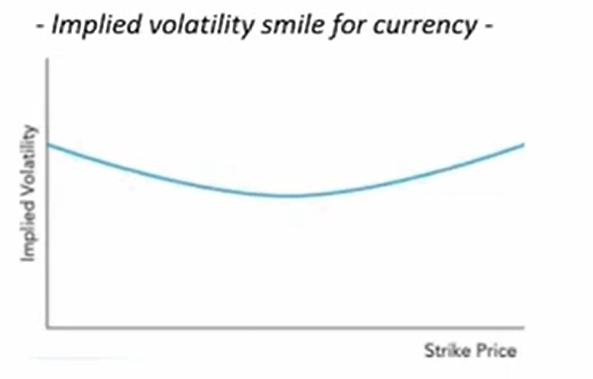
\includegraphics[width=.8\linewidth]{impl vol curr.PNG}
  \captionof{figure}{Валютные опционы}
  \label{fig:test1}
\end{minipage}%
\begin{minipage}{.5\textwidth}
  \centering
  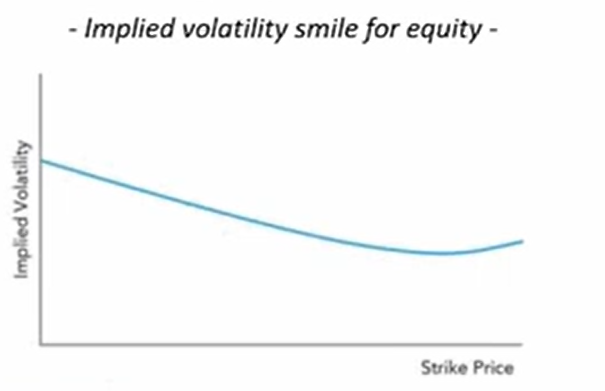
\includegraphics[width=.8\linewidth]{impl vol equity.PNG}
  \captionof{figure}{Опционы на акции}
  \label{fig:test2}
\end{minipage}
\end{figure}


\section{Влияние дивидендных платежей}
Ослабим условие на наличие дивидендов в БА \textit{(5)}.\\
В случае \textbf{непрерывных} дивидендов цены приобретают вид:

\begin{equation}
\begin{gathered}
c=S_0e^{-qt}N\left(d_1\right)-K e^{-r T} N\left(d_2\right) \\
p=K e^{-r T}N\left(-d_2\right)-S_0e^{-qt}N\left(-d_1\right) \\
\end{gathered}
\end{equation}\\
Здесь $q$ - сложная суммарная ставка дивиденда\\
В случае \textbf{дискретных дивидендов}: Пусть $D$ - \textit{present value} дивидендов, которые выплатят за период жизни опциона. Разобъём цену опциона $S$ на две составляющие
\begin{itemize}
    \item Выплачиваемую дивидендную часть $D$
    \item Часть $S-D$, которая останется на момент экспирации $T$. Эта часть будет учитываться в уравнении БШМ, и к ней будет применяться вменённая волатильность $\sigma$. Таким образом, цена БА на начальный момент времени $S_0-D$
\end{itemize}

\section{Опционы на валютные пары и фьючерсы}
\textbf{Валюту} можно рассматривать как акцию, на которую выплачиваются дивиденды по безрисковой ставке центробанка страны-эмитента валюты $r_f$. В этом случае $q=r_f$, и уравнение БШМ примет вид:
\begin{equation*}
\begin{gathered}
c=S_0 e^{-r_f T} N\left(d_1\right)-K e^{-r T} N\left(d_2\right) \\
p=K e^{-r T} N\left(-d_2\right)-S_0 e^{-r_f T} N\left(-d_1\right) \\
d_1=\frac{\ln \left(\frac{S_0}{K}\right)+\left(r-r_f+0.5 \sigma^2\right) T}{\sigma \sqrt{T}}, \\
d_2=\frac{\ln \left(\frac{S_0}{K}\right)+\left(r-r_f-0.5 \sigma^2\right) T}{\sigma \sqrt{T}}=d_1-\sigma \sqrt{T},
\end{gathered}
\end{equation*}\\
\textbf{Фьючерсы} в модели БШМ ведут себя аналогично валюте. В этом случае $q=r$, и уравнение БШМ:\\
\begin{equation*}
\begin{gathered}
c=F_0 e^{-r T} N\left(d_1\right)-K e^{-r T} N\left(d_2\right) \\
p=K e^{-r T} N\left(-d_2\right)-F_0 e^{-r T} N\left(-d_1\right) \\
d_1=\frac{\ln \left(\frac{F_0}{K}\right)+\sigma^2\frac{T}{2}}{\sigma \sqrt{T}}, \\
d_2=\frac{\ln \left(\frac{F_0}{K}\right)+\sigma^2\frac{T}{2}}{\sigma \sqrt{T}}=d_1-\sigma \sqrt{T},
\end{gathered}
\end{equation*}\\
\section{Американские опционы}
Ослабим теперь ограничение \textit{(8)}. Позиция в американском опционе без дивидендов аналогична позиции в европейском опционе без дивидендов. Рассмотрим американский опцион с дивидендными выплатами:\\
Предположим, что на БА выплачиваются дискретные дивиденды $D_i$ во времена $t_i$, при времени до экспирации опциона $T$. Тогда в момент времени $t_i$ неисполненная цена опциона составляет $S(t_i)-D_i-Ke^{-r(t_i+1-t_i)}$. Отсюда получаем, что опцион имеет смысл исполнять только при
\begin{equation*}
    S(t_i)-X>S(t_i)-D_i-Ke^{-r(t_i+1-t_i)}
\end{equation*}
Если идти от противного, получим условие, при котором опцион никогда не будет исполнен:
\begin{equation*}
\mathrm{D}_i \leq K\left(1-e^{-r\left(t_{i+1}-t_i\right)}\right) \text { и } \mathrm{D}_n \leq K\left(1-e^{-r\left(T-t_n\right)}\right)
\end{equation*}
При условии достаточной малости, когда верхние неравенства выполняются, американские опционы эквивалентны европейским.
\textbf{Аппроксимация Блэка} для американских аукционов заключается в вычислении стоимости двух эквивалентных европейских опционов, сроки действия которых истекают в момент экспирации $Т$ и момент последнего дивидендного платежа перед экспирацией $t_n$. Cтоимость американского опциона приравнивается к стоимости более дорогого европейского опциона. В большинстве случаев этот алгоритм даёт достаточно точные оценки.
\section{Оценка варрантов}
\textbf{Варрант} - обязательство, выпускаемое компанией на собственные акции. При исполнении варранта компания производит допэмиссию акций и продаёт их держателям варрантов по цене страйка, что приводит к размытию акционерного капитала.\\
Оценить варрант можно также при помощи модели БШМ. Принципиальное отличие заключается в наличии размытия капитала при исполнении контракта, и как следствие, падения цены акций. Стоимость варранта для держателей текущих акций зависит от степени размытия капитала: $\frac{pN}{N+M}$, где $p$ - цена варранта, рассчитанная через БШМ, $N$ - кол-во акций в обращении, $M$ - кол-во выпускаемых акций.
\end{document}
